% Options for packages loaded elsewhere
\PassOptionsToPackage{unicode}{hyperref}
\PassOptionsToPackage{hyphens}{url}
%
\documentclass[
]{article}
\usepackage{amsmath,amssymb}
\usepackage{lmodern}
\usepackage{iftex}
\ifPDFTeX
  \usepackage[T1]{fontenc}
  \usepackage[utf8]{inputenc}
  \usepackage{textcomp} % provide euro and other symbols
\else % if luatex or xetex
  \usepackage{unicode-math}
  \defaultfontfeatures{Scale=MatchLowercase}
  \defaultfontfeatures[\rmfamily]{Ligatures=TeX,Scale=1}
\fi
% Use upquote if available, for straight quotes in verbatim environments
\IfFileExists{upquote.sty}{\usepackage{upquote}}{}
\IfFileExists{microtype.sty}{% use microtype if available
  \usepackage[]{microtype}
  \UseMicrotypeSet[protrusion]{basicmath} % disable protrusion for tt fonts
}{}
\makeatletter
\@ifundefined{KOMAClassName}{% if non-KOMA class
  \IfFileExists{parskip.sty}{%
    \usepackage{parskip}
  }{% else
    \setlength{\parindent}{0pt}
    \setlength{\parskip}{6pt plus 2pt minus 1pt}}
}{% if KOMA class
  \KOMAoptions{parskip=half}}
\makeatother
\usepackage{xcolor}
\usepackage[margin=1in]{geometry}
\usepackage{graphicx}
\makeatletter
\def\maxwidth{\ifdim\Gin@nat@width>\linewidth\linewidth\else\Gin@nat@width\fi}
\def\maxheight{\ifdim\Gin@nat@height>\textheight\textheight\else\Gin@nat@height\fi}
\makeatother
% Scale images if necessary, so that they will not overflow the page
% margins by default, and it is still possible to overwrite the defaults
% using explicit options in \includegraphics[width, height, ...]{}
\setkeys{Gin}{width=\maxwidth,height=\maxheight,keepaspectratio}
% Set default figure placement to htbp
\makeatletter
\def\fps@figure{htbp}
\makeatother
\setlength{\emergencystretch}{3em} % prevent overfull lines
\providecommand{\tightlist}{%
  \setlength{\itemsep}{0pt}\setlength{\parskip}{0pt}}
\setcounter{secnumdepth}{-\maxdimen} % remove section numbering
\newlength{\cslhangindent}
\setlength{\cslhangindent}{1.5em}
\newlength{\csllabelwidth}
\setlength{\csllabelwidth}{3em}
\newlength{\cslentryspacingunit} % times entry-spacing
\setlength{\cslentryspacingunit}{\parskip}
\newenvironment{CSLReferences}[2] % #1 hanging-ident, #2 entry spacing
 {% don't indent paragraphs
  \setlength{\parindent}{0pt}
  % turn on hanging indent if param 1 is 1
  \ifodd #1
  \let\oldpar\par
  \def\par{\hangindent=\cslhangindent\oldpar}
  \fi
  % set entry spacing
  \setlength{\parskip}{#2\cslentryspacingunit}
 }%
 {}
\usepackage{calc}
\newcommand{\CSLBlock}[1]{#1\hfill\break}
\newcommand{\CSLLeftMargin}[1]{\parbox[t]{\csllabelwidth}{#1}}
\newcommand{\CSLRightInline}[1]{\parbox[t]{\linewidth - \csllabelwidth}{#1}\break}
\newcommand{\CSLIndent}[1]{\hspace{\cslhangindent}#1}
\ifLuaTeX
  \usepackage{selnolig}  % disable illegal ligatures
\fi
\IfFileExists{bookmark.sty}{\usepackage{bookmark}}{\usepackage{hyperref}}
\IfFileExists{xurl.sty}{\usepackage{xurl}}{} % add URL line breaks if available
\urlstyle{same} % disable monospaced font for URLs
\hypersetup{
  pdftitle={Normalizations are not what you think; Explicit Scale Simulation in ALDEx2},
  hidelinks,
  pdfcreator={LaTeX via pandoc}}

\title{Normalizations are not what you think; Explicit Scale Simulation
in ALDEx2}
\author{true \and true \and true}
\date{}

\begin{document}
\maketitle
\begin{abstract}
In many high-throughput sequencing (HTS) studies, sample-to-sample
variation in sequencing depth is not driven by variation in the scale
(e.g., total size, microbial load, or total gene expression) of the
underlying biological systems being measured but rather is driven by
technical factors. Typically the technical variation is addressed using
some form of statistical normalization. Normalizations are data or
parameter transformations that remove unwanted technical variation in
the hopes of facilitating analyses sensitive to scale; e.g.,
differential abundance and differential expression analyses. Recently we
showed that any normalization makes implicit assumptions about the
unmeasured system scale and that errors in these assumptions can lead to
dramatic increases in false positive and false negative rates. Here we
describe updates to the ALDEx2 R package that mitigate these problems by
directly modeling uncertainty in the unmeasured system scale through the
use of a \textit{scale model}. Scale models generalize the idea of
normalizations and can be thought of as explicitly modeling potential
error in the chosen normalization. Beyond enhancing the robustness of
HTS analyses, the use of scale models within ALDEx2 enhances the
transparency and reproducibility of analyses by making implicit
normalizing assumptions an explicit part of the model building process.
\end{abstract}

\hypertarget{introduction}{%
\section{Introduction}\label{introduction}}

High-throughput sequencing (HTS) is a ubiquitous tool used to explore
many biological phenomenon such as gene expression (single-cell
sequencing, RNA-sequencing, meta-transcriptomics), microbial community
composition (16S rRNA gene sequencing, shotgun metagenomics) and
differential enzyme activity (selex, CRISPR killing). HTS proceeds by
taking a sample from the environment, making a library, multiplexing
(merging) multiple libraries together, and then applying a sample of the
multiplexed library to the flow cell. Each of these steps can be though
of as a sampling step: a pool of DNA that could be measured is sampled
and only that subsampled DNA is carried over to subsequent steps. Within
each sampling step, the connection between the size of the sampled DNA
pool and the scale (e.g., size, microbial load, or total gene
expression) of the measured biological system is degraded or lost.
Increasingly, researchers are turning to modified experimental protocols
(e.g., DNA spike-ins or cell counting) in an attempt to recover the lost
biological variation in scale; see for example (Vandeputte et al. 2017;
Props et al. 2017). However, these protocols often do not recover
meaningful biological variation but instead recover scale variation at
some intermediate step in the sample preparation protocol (e.g., at the
stage where the DNA spike-in was added). In short, the disconnect
between sample-to-sample variation in sequencing depth and biological
variation in scale remains an outstanding challenge.

Biological variation in scale can represent an important unmeasured
confounder in HTS analyses (Lovell et al. 2015). For example, cells
transformed by the cMyc oncogene have about 3 times the amount of mRNA
and about twice the rRNA content than non-transformed cells (Nie et al.
2012), and this dramatically skews transcriptome analysis (Lovén et al.
2012). In addition, wild-type and mutant strains of cell lines, yeast or
bacteria often have different growth rates, which would affect our
ability to identify truly differentially abundant genes (Yoshikawa et
al. 2011). As another example, the total bacterial load of the vaginal
microbiome differs by 1-2 orders of magnitude in absolute abundance
between the healthy and bacterial vaginosis states (Zozaya-Hinchliffe et
al. 2010), and the composition between these states is dramatically
different (Ravel et al. 2011; Hummelen et al. 2010). Thus, a full
description of these systems includes both relative change (composition)
and absolute abundance (scale), yet current methods access only the
compositional information.

To be more concrete, let \(\mathbf{Y}\) denote an \(D \times N\) matrix
of sequence counts with elements \(\mathbf{Y}_{dn}\) denoting the number
of measured DNA molecules mapping to feature \(d\) (e.g., a taxon or
gene) in sample \(n\). Let \(\mathbf{W}\) also represent a
\(D \times N\) matrix but with elements \(\mathbf{W}_{dn}\) representing
the true (as opposed to measured) amount of class \(d\) in the
biological system from which sample \(n\) was obtained. Succinctly,
\(\mathbf{Y}\) denotes the observed HTS data whereas \(\mathbf{W}\)
denotes the true counts in the system under study. We can think of
\(\mathbf{W}\) as consisting of two parts, the scale
\(\mathbf{W}^{\perp}\) (e.g., totals) and the composition
\(\mathbf{W}^{\parallel}\) (i.e., proportions). That is,
\(\mathbf{W}^{\perp}\) is a \(N\)-vector with elements
\(\mathbf{W}^{\perp}_{n}=\sum_{d}\mathbf{W}_{dn}\) while
\(\mathbf{W}^{\parallel}\) is a \(D \times N\) matrix with elements
\(\mathbf{W}^{\parallel}_{dn}=\mathbf{W}_{dn}/\mathbf{W}^{\perp}_{n}\).
Note that with these definitions \(\mathbf{W}\) can be written as the
element-wise combination of scale and composition:
\(\mathbf{W}_{dn}=\mathbf{W}^{\parallel}_{dn}\mathbf{W}^{\perp}_{n}\).
The technical variation in sequencing depth
(\(\mathbf{Y}^{\perp}_{n}=\sum_{d}\mathbf{Y}_{dn}\)) implies that
observed data \(\mathbf{Y}\) provides us with information about the
system composition \(\mathbf{W}^{\parallel}\) but little to no
information in the system scale \(\mathbf{W}^{\perp}\) (Lovell et
al.~2011).

Early on, researchers recognized the potential confounding effects of
the non-biological variation in sequencing depth and approached the
problem using various forms of \textit{normalization}. The idea of
normalization is to remove this variation thus making the samples
commensurate and to correct any minor asymmetries in the data. A large
number of normalizations were developed. Rarefaction (Hughes and
Hellmann 2005) was used in the microbiome field, while transcriptome
investigators developed and used proportions and derivatives (reads per
kilobase per million, and transcripts per kilobase per million)
(Mortazavi et al. 2008; Wagner, Kin, and Lynch 2012), the relative log
expression (RLE) (Anders and Huber 2010) and trimmed mean of M values
(TMM) (Robinson and Oshlack 2010). The Centered Log Ratio (CLR)
(Aitchison 1982) was proposed as a unifying normalization (Fernandes et
al. 2014). With the exception of rarefaction, all of these
normalizations are data transformations that can be stated as ratios of
the form \(\hat{\mathbf{Y}}_{dn}=\mathbf{Y}_{dn}/f(\mathbf{Y})\); the
major differences being how the denominator is chosen and whether the
ratio is subsequently always log-transformed or not.

Recently, Nixon et al. (2023) suggested that the challenge of
non-biological variation in sequencing depth be viewed as a problem of
partially-identified models. Through this lens, they showed that
\emph{all} normalizations make some assumption about the system scale
\(\mathbf{W}^{\perp}\) in order to identify the chosen model. Moreover,
these assumptions are often implicit, difficult to interpret, and
provided different outputs when applied to the same dataset (Dillies et
al. 2013; Weiss et al. 2017). Intuitively, normalizations in widespread
use assume that either one sample can be chosen as a reference to which
the others are scaled (TMM), or that different sub-parts of each sample
maintain a constant scale across samples (RLE, CLR and derivatives).
Further, Nixon et al. (2023) showed that the original ALDEx2 model made
a strict assumption about scale through the CLR normalization. They
showed that this assumption could be remedied since ALDEx2 permits scale
to be easily incorporated into its framework. In this paper, we discuss
these modifications and show how including scale uncertainty can greatly
improve modeling and lead to more robust and reproducible results.

\hypertarget{adding-scale-uncertainty-in-aldex2}{%
\subsection{Adding Scale Uncertainty in
ALDEx2}\label{adding-scale-uncertainty-in-aldex2}}

The ALDEx2 R package (Fernandes et al. 2013) is a general purpose
toolbox for Bayesian modeling of HTS data. For brevity and concreteness,
we discuss ALDEx2 in its simplest form as a tool for estimating
Log-Fold-Changes (LFC) (e.g., differential abundance or differential
expression analysis), but note that it can be used to fit more complex
linear models. At a high-level, ALDEx2 involves three steps: 1) a
Bayesian model is used to estimate \(\mathbf{W}^{\parallel}\) given
observations \(\mathbf{Y}\); 2) a normalization is used to estimate
\(\mathbf{W}\) given the estimate \(\mathbf{W}^{\parallel}\); 3) the
\(\mathbf{W}\) estimates are used to estimate LFC as part of
differential abundance (or expression) analyses. For more details on
ALDEx2 see Fernandes et al. (2013).

By default, ALDEx2 uses the CLR normalization which can be written as
\(\log \mathbf{W}_{dn}=\log [\mathbf{W}^{\parallel}_{dn}/G_{n}]\) where
\(G_{n}\) denotes the geometric mean of the vector
\((W^{\parallel}_{1n}, \dots, W^{\parallel}_{Dn})\) (see Supplemental
Materials for how the CLR connects to Shannon entropy). Nixon et
al.~(2023) showed that in this context the CLR normalization equates to
an implicit assumption that \(\mathbf{W}^{\perp}_{n}=1/G_{n}\). They
showed that even slight errors in this assumption introduced bias into
LFC estimate that was not accounted for in estimates of uncertainty
(e.g., confidence intervals or credible sets). In fact, they showed that
the only way in which the ALDEx2 model, or any model that uses
normalizations, could ever be calibrated (e.g., control Type-I Error
rates) was if this assumption was exactly true. While this assumption
may be approximately correct in some instances it is surely never
exactly true. In support of this assertion it is known that false
discovery rates vary widely by analysis and normalization method
(Hawinkel et al. 2018; Li et al. 2022). As a result, Nixon et al.~(2023)
suggested that models should consider potential error in the assumptions
implied by normalizations.

Nixon et al.~(2023) proposed the concept of a \textit{scale model} as a
generalization of normalizations that account for potential error. They
showed how scale models can be incorporated into ALDEx2, turning the
ALDEx2 model into a specialized type of statistical model which they
called a \textit{Scale Simulation Random   Variable} (SSRV). Recall that
\(\mathbf{W}_{dn}=\mathbf{W}^{\parallel}_{dn}\mathbf{W}^{\perp}_{n}\).
As the HTS data only informs directly on
\(\mathbf{W}^{\parallel}_{dn}\), they proposed to augment analyses with
a model for \(\mathbf{W}^{\perp}_{n}\) (the scale model). Since the CLR
normalization makes the assumption \(\mathbf{W}^{\perp}_{n}=1/G_{n}\),
the CLR normalization can be generalized by considering probability
models for the scale \(\mathbf{W}^{\perp}_{n}\) that have mean
\(1/G_{n}\). For example, the following scale model generalizes the CLR:

\[\log \mathbf{W}^{\perp}_{n} = -\log G_{n} + \Lambda x_{n} \qquad \Lambda \sim N(0, \gamma^{2})\]

where \(\gamma\) is a tunable parameter that controls the degree of
uncertainty in the CLR assumption and \(x_{n}\) denotes a binary
condition indicator (e.g., \(x_{n}=1\) denotes case and \(x_{n}=0\)
denotes control). Beyond theoretical studies, they demonstrated through
the analysis of simulated and real data the remarkable performance
improvements that could result from incorporating this type of scale
uncertainty into analyses. Subsequently, we have made those
modifications a permanent fixture of ALDEx2 which now represents the
first software package designed for SSRV-based inference.

Beyond concerns of fidelity and rigor, scale models also enhance the
reproducibility and transparency of HTS analyses. This occurs because
rather than using an implicit assumption (e.g.,
\(\log \mathbf{W}^{\perp}=1/G_{n}\) for the CLR normalization), scale
models make this an explicit part of the model building process. While
it is beyond the scope of the present article, we note that there are
many ways of building scale models that enhance the interpretability of
the parameters and assumptions. Moreover, the scale model listed above,
which is now the default in ALDEx2, also has an appealing
interpretation. A detailed description of these points as well as the
mathematical underpinnings of the updated ALDEx2 R package is
forthcoming and will be made available as a companion publication. Here,
we simply treat the parameter \(\gamma\) in the default scale model as
an abstract term that represents uncertainty in the CLR assumption and
note that larger values of \(\gamma\) correspond to more uncertainty in
this assumption. We also show that the ratio of scales between
conditions can be used to build a full scale model when the conditions
have dramatically different underlying scales.

An advantage of incorporating scale is that analyses can be made much
more robust such that actual or potential differences in scale can be
tested and accounted for explicitly. The examples below and in the
supplement show how incorporating scale provides robust and
interpretable differential abundance estimates in several different
datasets.

\hypertarget{results}{%
\section{Results}\label{results}}

\hypertarget{adding-scale-uncertainty-replaces-the-need-for-dual-significance-cutoffs.}{%
\subsection{Adding scale uncertainty replaces the need for dual
significance
cutoffs.}\label{adding-scale-uncertainty-replaces-the-need-for-dual-significance-cutoffs.}}

Gierliński et al. (2015) conducted a highly replicated yeast
transcriptome experiment comparing a wild-type strain with a snf1 gene
knockout. This dataset has been used to argue that only a small number
of replicates are needed to identity differentially abundant genes and
makes the recommendation that some tools should be used in some
conditions because each tool has different intrinsic statistical power
and Type 1 and Type 2 errors (Schurch et al. 2016){]}. This guidance
runs counter to standard statistical practice where power is
intrinsically linked to sample size (Halsey et al. 2015), yet the
concept of sample-size independent power is entrenched in all fields
that use HTS as an experimental readout. Through the lens of this paper,
this is a hallmark of unacknowledged bias: a false certainty in the
scale of the data brings about an increasing false precision with
increasing sample sizes. Furthermore, the yeast transcriptome experiment
has an unacknowledged difference in scale between conditions: yeast
deficient for snf1 are smaller, grow more slowly and are sensitive to a
variety of common agents that cause cell stress (Yoshikawa et al. 2011).
Thus, by adding scale uncertainty, we can be more confident that the
results of the analysis reflect true biological differences and not
differences due to the assumptions made by the normalization method.

We start by examining the dispersion (variance) of the data as counts
and as the logarithm of the normalized counts when calculated by DESeq2
(log(RLE)) or by ALDEx2 (CLR). The raw data counts derived from
sequencing are overdispersed with the mean value being less than the
variance (Robinson and Oshlack 2010; Robinson, McCarthy, and Smyth 2010)
as seen in Panel A of Figure 1. However, the actual analysis of
differential abundance is performed on the logarithm of the normalized
counts (Robinson, McCarthy, and Smyth 2010; Love, Huber, and Anders
2014; Andrews and Hemberg 2019), which includes the CLR (Fernandes et
al. 2013) yet the mean-dispersion distribution of these log-ratio
transformed data is quite different as shown in panels B and C of Figure
1 and as noted elsewhere (Fernandes et al. 2013; Love, Huber, and Anders
2014).

\begin{figure}
\centering
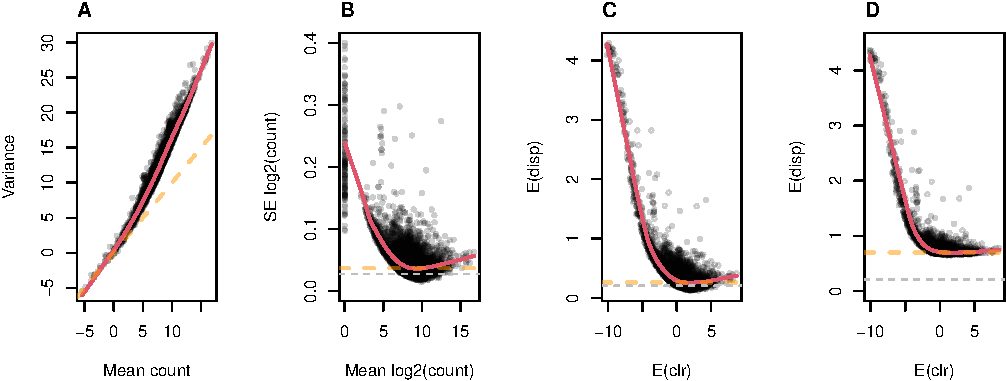
\includegraphics{go3_files/figure-latex/dispersion-1.pdf}
\caption{Plot of abundance v dispersion for a typical transcriptome
dataset as counts, as logarithms of counts, and as clr values. Panel A
shows that the data are over-dispersed relative to a Poisson
distribution which is represented by the dashed line when plotted on a
log-log scale. Panel B shows that the relationship between the mean and
the dispersion calculated in DESeq2, here the standard error (SE) of the
mean, is very different when the data are log-transformed first. Panel C
shows the equivalent values calculated by ALDEx2 in which the expected
clr value for each transcipt are plotted vs.~the expected dispersion.
The red line in each panel shows the loess line of fit to the mid-point
of the distributions. In panels B and C the amount of dispersion reaches
a minimum at moderate values. The dashed orange line in panel A is the
line of equivalence, and in panel B and C is the minimum y value. The
values below the dashed grey line in panels B and C represent those
below the first decile of dispersion.}
\end{figure}

These relationships depend on what is being analyzed: the variance or
dispersion always increases with increasing raw (or normalzied) read
count but decreases when measured on the log-ratio transformed data
(Fernandes et al. 2013; Love, Huber, and Anders 2014), reaching a
minimum at some mid-point of the distribution. This makes the
counter-intuitive suggestion that genes with moderate expression have
more predictable expression than genes with very high expression such as
housekeeping genes. This is at odds with the known biology of cells
where single cell counting of housekeeping transcripts shows that they
are both highly expressed and have little intrinsic variation (Taniguchi
et al. 2010). Furthermore, the dispersion is exceeding small being, for
many transcripts, almost negligible. To show this point more clearly,
the majority of the transcripts in the lowest decile of dispersion
indicated below the dashed grey line are statistically significantly
different (75\% with DESeq2, 69\% with ALDEx2), suggesting that low
dispersion estimates lead to many false positives. From the perspective
of Nixon et al. (2023), it is reasonable to conclude that some of these
results may be due to the choice of normalization. Indeed, benchmarking
and comparison studies have repeatedly shown that the choice of
normalization plays a role in which results are returned as significant;
see for example (Maza et al. 2013), (Dillies et al. 2013) and (Weiss et
al. 2017).

Using either DESeq2 or ALDEx2, a majority of transcripts are
statistically significantly different between groups even with a
Benjamini-Hochberg (Benjamini and Hochberg 1995) false discovery rate
(FDR) of 0.01; i.e.~4264 or 3790 of the 5891 transcripts are
statistically significant. Clearly, a 70\% positive rate seems
biologically unjustified, and furthermore this breaks the necessary
assumption made by the normalization methods that most features must be
invariant. Finally, that 90 transcripts are identified by ALDEx2 and not
DESeq2, while DESeq2 identifies 564 transcripts that ALDEx2 does not
suggests that the choice of normalization plays a role in which results
are returned as significant.

\begin{figure}
\centering
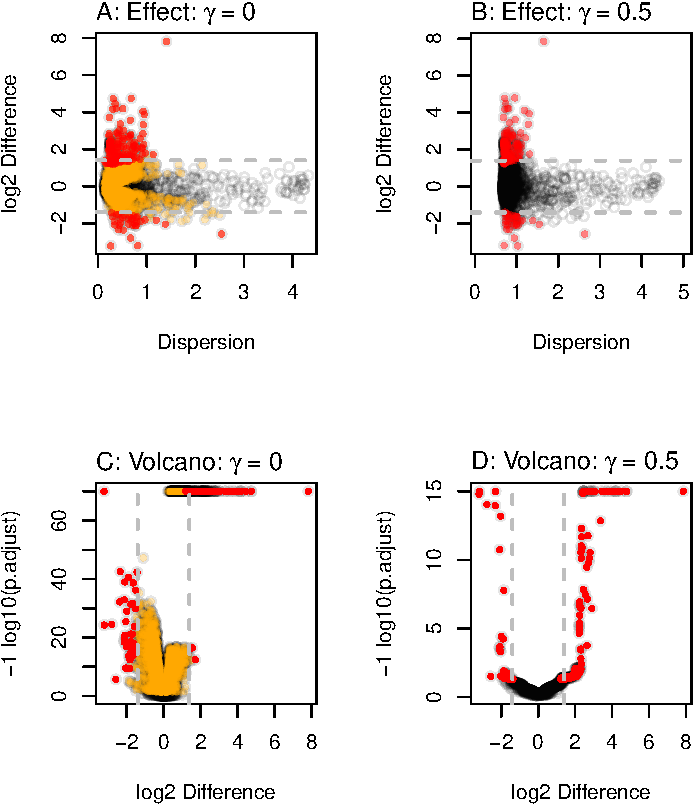
\includegraphics{go3_files/figure-latex/plot1-1.pdf}
\caption{Effect and volcano plots for unscaled and scaled transcriptome
analysis. DESeq2 or ALDEx2 were used to conduct a differential abundance
(DA) analysis on the yeast transcriptome dataset. The results were
plotted to show the relationship between difference and dispersion using
effect plots ) or difference and the Benjamini-Hochberg corrected
p-values (volcano plot). Panels A,B,D,E are for the unscaled analysis,
and Panels C,F are for the scaled analysis. Each point represents the
values for one transcript, with the color indicating if that transcript
was significant in the scaled analysis and unscaled analysis (red) or in
the unscaled analysis only (orange). Points in grey are not
statistically signficantly different with any analysis. The horizontal
dashed lines represent a log2(difference) of 1.4, which is a commonly
applied cutoff when the majority of features are statistically
significant.}
\end{figure}

As shown using effect (Gloor, Macklaim, and Fernandes 2016) and volcano
plots (Cui and Churchill 2003) in Figure 2 A,B,D,E, the root cause of
the many statistically significant positive transcripts is the very
large number of transcripts with negligible variance. This phenomenon is
shared between methods: almost all the transcripts that are
differentially abundant with an FDR \textless 0.01 (orange and red
points) have extremely low dispersion and a very low difference between
groups. In the most extreme cases, some transcripts have a near zero
difference between groups. This issue is not unique to this data set and
it is common practice to use a dual-cutoff by choosing transcripts based
on a thresholds for both corrected p-values and fold-changes (Schurch et
al. 2016) (commonly set at \(\pm 2^{1.4}\) for the latter). These limits
are shown by the dashed grey lines. In this case, applying a dual-cutoff
using a heuristic of at least a \(2^{1.4}\) fold change reduces the
number of significant outputs to 193 for DESeq2 and to 186 for ALDEx2.
This result begs the question: why bother with significance tests at
all?

The very low dispersion estimate for most features is a by-product of
sequencing and normalization. While the actual scale of the data is
inaccessible post-sequencing, we can study the sensitivity of the
results to the choice of normalization and thus scale. To do this we
incorporate scale models (Nixon et al. 2023) in lieu of normalizations
through the default scale model that is now built into ALDEx2. Scale
uncertainty is incorporated using the \texttt{gamma} parameter that
controls the amount uncertainty added to the CLR mean assumption when we
call either \texttt{aldex()}, or \texttt{aldex.clr()}. The
\texttt{ALDEx2} package further contains a sensitivity analysis
function, \texttt{aldex.senAnalysis()}, that can be used to explore the
effect of different amounts of scale uncertainty. In practice, we
suggest that a \texttt{gamma} parameter between 0.5 and 1 is realistic
for most experimental designs.

Applying the default scale model with \texttt{gamma=1}, a large number
of transcripts with near 0 dispersion have had their dispersion
increased (Figure 2C), and this results in many fewer transcripts 100
being called significantly different as shown in the volcano plot in
Figure 1F (red points). Furthermore, overplotting the significant
transcripts identified after adding scale uncertainty on the un-scaled
analysis shows that adding scale uncertainty removes the need for the
dual cutoff. Indeed, adding scale uncertainty reduces the significant
transcripts to a subset of those identified with the dual cutoff that
have the largest effect size. Thus, incorporating scale uncertainty
through the default scale model allows us to determine which variables
are likely to be significant due to sequencing and normalization, and
which are significantly different even with scale uncertainty included.

\hypertarget{housekeeping-genes-can-be-used-to-guide-scale-model-choices.}{%
\subsection{Housekeeping genes can be used to guide scale model
choices.}\label{housekeeping-genes-can-be-used-to-guide-scale-model-choices.}}

Macklaim and Gloor (2018) and Wu et al. (2021) used a vaginal
metatranscriptome dataset used to compare the gene expression in
bacteria collected from healthy (H) and bacterial vaginosis (BV)
affected women. In this environment, both the relative abundance of
species between groups and the gene expression level within a species is
different (Macklaim et al. 2013). Additionally, prior research suggests
that the total number of bacteria is about 10 times more in the BV than
in the H condition (Zozaya-Hinchliffe et al. 2010). Thus, this is an
extremely challenging environment in which to determine differential
abundance as there are both compositional and scale changes between
conditions. The accepted method to analyze vaginal metratranscriptome
data is on a taxon-by-taxon basis (Macklaim et al. 2013; Deng et al.
2018; Fettweis et al. 2019) because the scale confounding can be
ignored. The problem with a systemic analysis is that many housekeeping
genes are returned as differentially abundant between groups, a result
likely due to a disconnect between the scale assumptions of the
normalization used (Wu et al. 2021) and the actual change in scale
between conditions.

In this example, we show how to specify the scale model explicitly and
demonstrate that applying a user-defined scale model can account for
some of these modeling difficulties. A user-defined scale model can
control for both the mean difference of scale between groups (e.g.,
directly incorporate information on the differences in total number of
bacteria between the BV and H conditions) as well as the uncertainty
assumed in that difference. To specify a user-defined scale model, we
can pass a matrix of scale values instead of a single estimate of gamma
to \texttt{aldex.clr()}. This matrix should have the same number of rows
as the of Monte-Carlo Dirichlet samples, and the same number of columns
as the number of samples. While this matrix can be computed from scratch
by the analyst, there is an \texttt{aldex.makeScaleModel()} function
that can be used to simplify this step in most cases.

Figure 3A shows an effect plot (Gloor, Macklaim, and Fernandes 2016) of
the data where reads are grouped by function, corresponding
approximately to grouping orthologous sequences regardless of the
organism of origin. Each point represents one of the 3728 functions.
There are many more functions represented in the BV group (bottom) than
in the healthy group (top). This is because the \textit{Lactobacilli}
that dominate a healthy vaginal microbiome have reduced genome content
relative to the anaerobic organisms that dominate in BV, because there
is a greater diversity of organisms in BV than in H samples and because
the BV condition has at least an order of magnitude more bacteria than
does the H condition.

We can see that there are a large number of core metabolic and
information processing functions that are shared between the two groups
(boxed area in Figure 3A), and inspection shows that these largely
correspond to core metabolic functions that would not be expected to
contribute to differences in ecosystem behaviour and so should not be
differentially abundant. As a proxy for housekeeping functions the core
ribosome functions (blue) shows that their mean location is not centred
on 0. The major group of these housekeeping functions is located off the
line of no difference (being approximately located at +1.5). Since they
have very low dispersions, these functions are identified as
differentially abundant (red) along with many others. While changes in
the abundance of housekeeping functions is a useful proxy for relative
abundance of species in the environment, they tell us nothing about the
functional capacity of the two groups because these are functions in
common to every organism. Of more interest is determining the functions
that are different between groups because these are unique or
over-expressed in one group relative to the other.

\begin{figure}
\centering
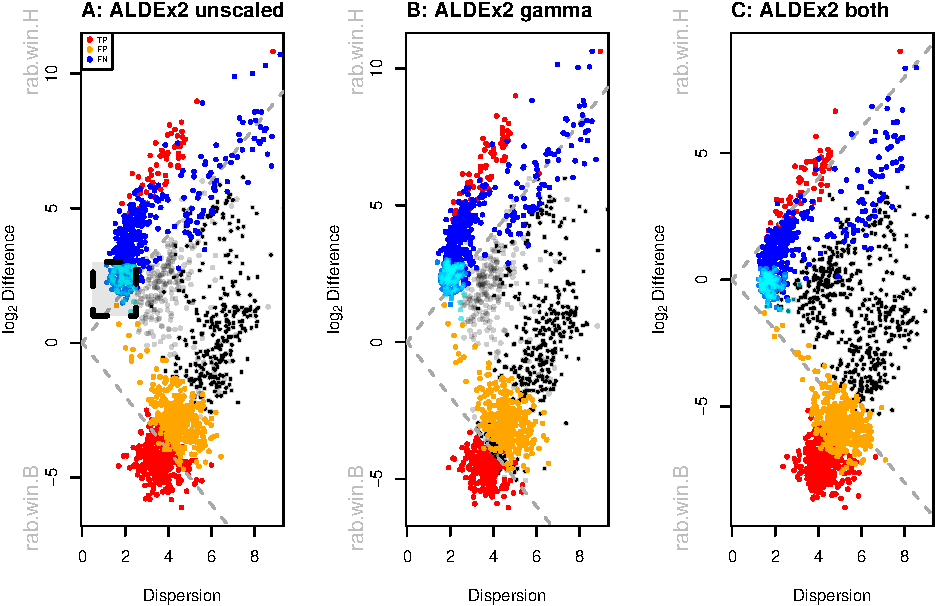
\includegraphics{go3_files/figure-latex/meta-1.pdf}
\caption{Analysis of vaginal transcriptome data aggregated at the Kegg
Orthology (KO) functional level. Panel A shows an effect plot for the
default analysis where the functions that are elevated in the healthy
individuals have positive values and functions that are elevated in BV
have negative values. Highlighed in the box are highly abundant KOs that
are almost exlusively housekeeping functions, with ribosomal KOs
highlighted in blue, statistically significant (FDR \textless{} 0.01)
functions in red, and non-significant functions in black or orange.
These housekeeping functions should be located on the midline of no
difference. Panel B shows the same data scaled with
\texttt{gamma\ =\ 0.5}, which increase the minimum dispersion
approximatly by one unit. Here the housekeeping functions from Panel A
are colored cyan or blue for reference. Panel C shows the same data
scaled with \texttt{gamma\ =\ 0.5} and a 0.15 fold difference in
dispersion applied to the BV samples relative to the H samples. The
orange functions are now statistically significant. Note that this
shifts the midpoint of the housekeeping functions towards the midline.}
\end{figure}

Applying the default scale model of \texttt{gamma=0.5} increases the
dispersion as expected but does little to move the large number of
housekeeping functions toward the midline of no difference. This is as
expected: the mean of the default scale model is based on the CLR
normalization so no shift would be expected over the original ALDEx2
model. Nevertheless, about 50\% of the housekeeping functions are no
longer statistically significantly different. Note that this change is
simple to conduct, has no additional computational complexity and
requires only a slight modification from the analyst.

Up to this point, scale uncertainty has been applied as an extension of
the CLR normalization via the default scale model, but a user-defined
scale adjustment can be applied to each condition, or even each sample
independently through a custom scale matrix. While not necessary in all
datasets (e.g., the transcriptome example discussed in the previous
section and see the Supplementary material), it can greatly improve
modeling in certain cases, especially when the scale is highly
asymmetric between conditions. In order to specify a scale model from
scratch, we need to revisit the concept that all normalizations in
widespread use are actually ratios with the denominator implied by the
normalization. Therefore, we can easily deviate from a certain
normalization (e.g., the geometric mean assumption implied by the CLR)
by specifying a total model based on the mean difference between
conditions. While knowing the mean difference between conditions may
seem cumbersome in practice, it is the \emph{relationship} between the
group scale values that is important, not their raw values (Nixon et
al.~2023). This can be illustrated quite simply by starting with the
mean ratio in \(G\) between groups for the yeast transcriptome dataset
which are \(6.05\times 10^{-5}\) for snf2 and \(5.08\times 10^{-5}\) for
WT; their ratio being 1.17, or a 0.17-fold difference. Using this
information, we can recapitulate the differential abundance analysis in
Figure 2B and 2C exactly by using setting the mean denominator of group
1 to 1, and group 2 to 1.17 with a gamma of 0.5 as shown in Supplemental
Figure 2. This ratio can be adjusted to alter the mean assumption placed
on the group scale values.

With this background, we can understand how to apply a user-defined
scale model to the metratranscriptome dataset. While a user-defined
scale model can be quite flexible with relative scales that are distinct
for each group (or even each sample) along with their uncertainties,
here we focus on using the \texttt{aldex.makeScaleMatrix()} function.
This function uses a logNormal distribution to build a scale matrix
given a user-specified mean difference between groups and uncertainty
level. Applying a per-group relative differential scale of 0.15 moves
the housekeeping functions to the midline of no difference, and applying
a gamma of 0.5 provides the same dispersion as using a gamma of 0.5 with
the CLR (Figure 3C). Note that now a significant number of functions are
differentially up in BV that were formerly classed as not different
without scale, or when only a default scale was applied. These former
false negatives are noted in orange in each panel. Inspection of the
functions shows that these are largely missing from the Lactobacillus
species and so should actually be captured as differentially abundant.
Thus, applying a differential scale allows us to distinguish between
both false positives (housekeeping functions in cyan) and false
negatives (orange functions) even in a very difficult to analyze
dataset. We suggest that the default scale model is sufficient when the
data are approximately centred. However, when datasets are not well
centred or when the investigator has prior information about the
underlying biology, we advocate developing and using a user-specified
scale model.

\hypertarget{discussion}{%
\section{Discussion}\label{discussion}}

Biological count data derived from HTS can be decomposed into two parts:
the relative (compositional) and the absolute (scale), and the product
of these generates a fully scaled biological system (Nixon et al.~2023).
Biological systems are both predictably variable and stochastic, and
current measurement methods that rely on high throughput sequencing fail
to capture all of that variation, particularly variation due to scale.
In the absence of information external to the sequencing run itself, no
normalisation method can recapture any of the scale information (Lovén
et al.~2012). Even so, many methods such as flow cytometry (Vandeputte
et al.~2017), spike-in probes and fluorescent in-situ hybridization
(Lovén et al.~2012; Marguerat et al.~2012) have been proposed as a means
to do this. In the context of the updated ALDEx2 software suite, these
methods can be useful if they contain information on the particular
scale the researcher is interested in.

The ALDEx2 R package is readily amenable for incorporating scale
uncertainty. Originally, this tool used the only the Dirichlet
distribution to sample compositional uncertainty. Rather than applying
the CLR normalization as in the original ALDEx2, scale uncertainty can
be added through the use of a scale model with no additional
computational complexity. Scale uncertainty can be sampled from any
distribution depending on prior knowledge or preference. By default,
ALDEx2 samples scale from a logNormal distribution inspired by the CLR
normalization. However, there is the option to introduce a full scale
model that encapsulates both uncertainty and asymmetry in underlying
scale.

All normalizations attempt to make the samples in a dataset commensurate
but do not explicitly address the scale of the underlying system. The
two supplementary tables show that these normalizations can be
interpreted as scale assumptions. However, the general lack of scale
information has important consequences for the analysis of HTS datasets.
One issue is that analysis tools seem over-powered with even moderate
sample sizes, and different tools have different intrinsic power, Type 1
and Type 2 error rates (Schurch et al.~2016) and fail to account for
false discovery rates properly (Hawinkel et al. 2018; Li et al. 2022).
Traditional recommendations would suggest that using small sample sizes
in analysis leads to less reliability and reproducibility in analyses
since surprisingly large sample sizes are needed to determine
reproducible p-values (e.g., Halsey et al. (2015)). However,
recommendations to use small sample sizes are widespread in multivariate
datasets such as RNA-seq datasets. We argue that this is a hallmark of
unacknowledged bias: since normalizations are typically assumed to be
correct with no uncertainty, smaller samples offer an unintentional
buffer against this misspecification. Another issue is that datasets are
difficult to analyze when they contain systematic asymmetry, with
different tools exhibiting differing pathologies with these datasets
(Robinson and Oshlack 2010; Wu et al. 2021).

Many groups have conducted benchmarking studies on different tools and
normalizations used for the analysis of datasets such as transcriptomes
(Bullard et al. 2010; Soneson and Delorenzi 2013; Schurch et al. 2016;
Quinn, Crowley, and Richardson 2018) and microbiomes (Thorsen et al.
2016; Weiss et al. 2017; Hawinkel et al. 2018). Generically, it is
observed that the actual agreement between methods can be modest, and
there is usually a recommendation that some methods are better suited
for individual datasets or for specific types of analysis;
e.g.,\textasciitilde`Normalization and microbial differential abundance
strategies depend upon data characteristics' (Weiss et al. 2017).{]}
However, another interpretation of such studies is that different
normalizations can be better suited to different datasets by
happenstance, but it is not obvious how the use of specific
normalizations could be justified on a per dataset basis. There are now
published examples of multiple large replication efforts in psychology
(Open Science Collaboration 2015), cancer biology (Rodgers and Collings
2021), ecology and evolution (Gould and et.al 2023). In a nutshell,
experiences from these studies indicate that published data typically
have higher effect sizes and appear more significant than replication
efforts with the same data, or with newly generated replication data
(Rodgers and Collings 2021). Thus, most published data should be viewed
with suspicion (Ioannidis 2005) unless efforts have been made to ensure
that the results are robust.

In the case of overpowering, HTS analyses seem to be more robust when
applying a dual cutoff of both p-value and difference between group
means (Schurch et al. 2016). Figure 2 shows one reason for this
robustness could be that the dual cutoff is mimicking the effect of
including scale uncertainty, since substantially similar transcripts are
identified by the two approaches. We believe that adding scale
uncertainty leads to a more transparent analysis compared to the cutoff
as it is easy to describe the conditions under which certain conclusions
hold. Furthermore, while using the post-hoc difference cutoff is useful
for differential abundance analysis, it is not clear how this can be
incorporated into other kinds of downstream analyses. Conversely,
analyses that include scale uncertainty are fully compatible with
existing downstream analyses.

In the case of asymmetry, the use of a user-specified scale model can be
very useful for otherwise difficult-to-analyze datasets such as
meta-transcriptomes and in-vitro selection datasets where the majority
of features can change. We showed one such example in Figure 3 where the
dataset was highly asymmetrical, and the TMM and RLE normalizations
cannot fully move all the housekeeping genes to the midline of no
difference or exhibit other pathologies (Supplemental). Incorporating
differential scale on a per-group basis moves the mass of the data
towards the midline of no difference and so affects both Type I and Type
II error rates. In this analysis, transcripts that were previously not
classed as differentially abundant are now called as significantly
different, and the housekeeping transcripts move from being
significantly different to not being identified as such. While we
acknowledge that some prior information on which housekeeping
transcripts should not be classed as DA is needed, we suggest that this
information is widely available and is already used when performing the
gold-standard quantitative PCR test of differential abundance (Thellin
et al. 1999; SEQC/MAQC-III Consortium 2014). Furthermore, the assumption
that housekeeping genes should not generally be included in differential
abundance analysis is implicit in the dual p-value, fold-change cutoff
approach in widespread use. Thus, the use of this prior knowledge is not
unique to our approach.

In summary, while the underlying scale of the system is generally
inaccessible, the effect of scale on the analysis outcomes can be
modelled and can help explain some of the underlying biology. Adding
scale information to the analysis allows for more robust inference
because the features that are sensitive to scale can be identified and
their impact on the analysis weighted accordingly. Additionally, the use
of user-defined scale models permits difficult to analyze datasets to be
examined in a robust and principled manner even when the majority of
features are asymmetrically distributed or expressed (or both) in the
groups. Thus, reporting scale uncertainty should become a standard
practice in the analysis of HTS datasets as a way to identify which
features are most robust to differences in the underlying system.
Finally, we supply a toolkit that makes incorporating scale simple even
for datasets that come from highly asymmetrical environments.

\hypertarget{references}{%
\section*{References}\label{references}}
\addcontentsline{toc}{section}{References}

\hypertarget{refs}{}
\begin{CSLReferences}{1}{0}
\leavevmode\vadjust pre{\hypertarget{ref-aitchison1982}{}}%
Aitchison, John. 1982. {``The Statistical Analysis of Compositional
Data.''} \emph{Journal of the Royal Statistical Society: Series B
(Methodological)} 44 (2): 139--60.

\leavevmode\vadjust pre{\hypertarget{ref-Anders:2010}{}}%
Anders, Simon, and Wolfgang Huber. 2010. {``Differential Expression
Analysis for Sequence Count Data.''} \emph{Genome Biol} 11 (10): R106.
\url{https://doi.org/10.1186/gb-2010-11-10-r106}.

\leavevmode\vadjust pre{\hypertarget{ref-Andrews:2019aa}{}}%
Andrews, Tallulah S, and Martin Hemberg. 2019. {``M3Drop: Dropout-Based
Feature Selection for scRNASeq.''} \emph{Bioinformatics} 35 (16):
2865--67. \url{https://doi.org/10.1093/bioinformatics/bty1044}.

\leavevmode\vadjust pre{\hypertarget{ref-benjamini:1995}{}}%
Benjamini, Yoav, and Yosef Hochberg. 1995. {``Controlling the False
Discovery Rate: A Practical and Powerful Approach to Multiple
Testing.''} \emph{Journal of the Royal Statistical Society. Series B
(Methodological)} 57 (1): 289--300.

\leavevmode\vadjust pre{\hypertarget{ref-Bullard:2010}{}}%
Bullard, James H, Elizabeth Purdom, Kasper D Hansen, and Sandrine
Dudoit. 2010. {``Evaluation of Statistical Methods for Normalization and
Differential Expression in m{RNA-Seq} Experiments.''} \emph{BMC
Bioinformatics} 11: 94. \url{https://doi.org/10.1186/1471-2105-11-94}.

\leavevmode\vadjust pre{\hypertarget{ref-Cui:2003aa}{}}%
Cui, Xiangqin, and Gary A Churchill. 2003.
{``\href{https://www.ncbi.nlm.nih.gov/pubmed/12702200}{Statistical Tests
for Differential Expression in cDNA Microarray Experiments}.''}
\emph{Genome Biol} 4 (4): 210.1--10.

\leavevmode\vadjust pre{\hypertarget{ref-Denge00262-18}{}}%
Deng, Zhi-Luo, Cornelia Gottschick, Sabin Bhuju, Clarissa Masur,
Christoph Abels, and Irene Wagner-Döbler. 2018. {``Metatranscriptome
Analysis of the Vaginal Microbiota Reveals Potential Mechanisms for
Protection Against Metronidazole in Bacterial Vaginosis.''} Edited by
Craig D. Ellermeier, Janet Hill, and Andrew Onderdonk. \emph{mSphere} 3
(3). \url{https://doi.org/10.1128/mSphereDirect.00262-18}.

\leavevmode\vadjust pre{\hypertarget{ref-Dillies:2013}{}}%
Dillies, Marie-Agnès, Andrea Rau, Julie Aubert, Christelle
Hennequet-Antier, Marine Jeanmougin, Nicolas Servant, Céline Keime, et
al. 2013. {``A Comprehensive Evaluation of Normalization Methods for
{Illumina} High-Throughput {RNA} Sequencing Data Analysis.''}
\emph{Brief Bioinform} 14 (6): 671--83.
\url{https://doi.org/10.1093/bib/bbs046}.

\leavevmode\vadjust pre{\hypertarget{ref-fernandes:2013}{}}%
Fernandes, Andrew D, Jean M Macklaim, Thomas G Linn, Gregor Reid, and
Gregory B Gloor. 2013. {``ANOVA-Like Differential Expression (ALDEx)
Analysis for Mixed Population RNA-Seq.''} \emph{PLoS One} 8 (7): e67019.
\url{https://doi.org/10.1371/journal.pone.0067019}.

\leavevmode\vadjust pre{\hypertarget{ref-fernandes:2014}{}}%
Fernandes, Andrew D, Jennifer Ns Reid, Jean M Macklaim, Thomas A
McMurrough, David R Edgell, and Gregory B Gloor. 2014. {``Unifying the
Analysis of High-Throughput Sequencing Datasets: Characterizing
{RNA}-Seq, 16{S} r{RNA} Gene Sequencing and Selective Growth Experiments
by Compositional Data Analysis.''} \emph{Microbiome} 2: 15.1--13.
\url{https://doi.org/10.1186/2049-2618-2-15}.

\leavevmode\vadjust pre{\hypertarget{ref-Fettweis:2019aa}{}}%
Fettweis, Jennifer M, Myrna G Serrano, J Paul Brooks, David J Edwards,
Philippe H Girerd, Hardik I Parikh, Bernice Huang, et al. 2019. {``The
Vaginal Microbiome and Preterm Birth.''} \emph{Nat Med} 25 (6):
1012--21. \url{https://doi.org/10.1038/s41591-019-0450-2}.

\leavevmode\vadjust pre{\hypertarget{ref-Gierlinski:2015aa}{}}%
Gierliński, Marek, Christian Cole, Pietà Schofield, Nicholas J Schurch,
Alexander Sherstnev, Vijender Singh, Nicola Wrobel, et al. 2015.
{``Statistical Models for RNA-Seq Data Derived from a Two-Condition
48-Replicate Experiment.''} \emph{Bioinformatics} 31 (22): 3625--30.
\url{https://doi.org/10.1093/bioinformatics/btv425}.

\leavevmode\vadjust pre{\hypertarget{ref-gloor:effect}{}}%
Gloor, GB, JM Macklaim, and AD Fernandes. 2016. {``Displaying Variation
in Large Datasets: Plotting a Visual Summary of Effect Sizes.''}
\emph{Journal of Computational and Graphical Statistics} 25 (3C):
971--79. \url{https://doi.org/10.1080/10618600.2015.1131161}.

\leavevmode\vadjust pre{\hypertarget{ref-evoRepr-pre}{}}%
Gould, E, and et.al. 2023. {``Same Data, Different Analysts: Variation
in Effect Sizes Due to Analytical Decisions in Ecology and Evolutionary
Biology.''} \emph{EcoEvoRxiv}.
https://doi.org/\url{https://doi.org/10.32942/X2GG62}.

\leavevmode\vadjust pre{\hypertarget{ref-Halsey:2015aa}{}}%
Halsey, Lewis G, Douglas Curran-Everett, Sarah L Vowler, and Gordon B
Drummond. 2015. {``The Fickle p Value Generates Irreproducible
Results.''} \emph{Nat Methods} 12 (3): 179--85.
\url{https://doi.org/10.1038/nmeth.3288}.

\leavevmode\vadjust pre{\hypertarget{ref-hawinkel2017}{}}%
Hawinkel, Stijn, Federico Mattiello, Luc Bijnens, and Olivier Thas.
2018. {``A Broken Promise : Microbiome Differential Abundance Methods Do
Not Control the False Discovery Rate.''} \emph{BRIEFINGS IN
BIOINFORMATICS}. \url{http://dx.doi.org/10.1093/bib/bbx104}.

\leavevmode\vadjust pre{\hypertarget{ref-Hughes:2005tu}{}}%
Hughes, Jennifer B, and Jessica J Hellmann. 2005. {``The Application of
Rarefaction Techniques to Molecular Inventories of Microbial
Diversity.''} \emph{Methods Enzymol} 397: 292--308.
\url{https://doi.org/10.1016/S0076-6879(05)97017-1}.

\leavevmode\vadjust pre{\hypertarget{ref-Hummelen:2010}{}}%
Hummelen, Ruben, Andrew D Fernandes, Jean M Macklaim, Russell J Dickson,
John Changalucha, Gregory B Gloor, and Gregor Reid. 2010. {``Deep
Sequencing of the Vaginal Microbiota of Women with {HIV}.''} \emph{PLoS
One} 5 (8): e12078. \url{https://doi.org/10.1371/journal.pone.0012078}.

\leavevmode\vadjust pre{\hypertarget{ref-Ioannidis:2005aa}{}}%
Ioannidis, John P A. 2005. {``Why Most Published Research Findings Are
False.''} \emph{PLoS Med} 2 (8): e124.
\url{https://doi.org/10.1371/journal.pmed.0020124}.

\leavevmode\vadjust pre{\hypertarget{ref-Li:2022aa}{}}%
Li, Yumei, Xinzhou Ge, Fanglue Peng, Wei Li, and Jingyi Jessica Li.
2022. {``Exaggerated False Positives by Popular Differential Expression
Methods When Analyzing Human Population Samples.''} \emph{Genome Biol}
23 (1): 79. \url{https://doi.org/10.1186/s13059-022-02648-4}.

\leavevmode\vadjust pre{\hypertarget{ref-Love:2014aa}{}}%
Love, Michael I, Wolfgang Huber, and Simon Anders. 2014. {``Moderated
Estimation of Fold Change and Dispersion for RNA-Seq Data with
DESeq2.''} \emph{Genome Biol} 15 (12): 550.1--21.
\url{https://doi.org/10.1186/s13059-014-0550-8}.

\leavevmode\vadjust pre{\hypertarget{ref-Lovell:2015}{}}%
Lovell, David, Vera Pawlowsky-Glahn, Juan José Egozcue, Samuel
Marguerat, and Jürg Bähler. 2015. {``Proportionality: A Valid
Alternative to Correlation for Relative Data.''} \emph{PLoS Comput Biol}
11 (3): e1004075.
https://doi.org/\url{https://doi.org/10.1371/journal.pcbi.1004075}.

\leavevmode\vadjust pre{\hypertarget{ref-Loven:2012aa}{}}%
Lovén, Jakob, David A Orlando, Alla A Sigova, Charles Y Lin, Peter B
Rahl, Christopher B Burge, David L Levens, Tong Ihn Lee, and Richard A
Young. 2012. {``Revisiting Global Gene Expression Analysis.''}
\emph{Cell} 151 (3): 476--82.
\url{https://doi.org/10.1016/j.cell.2012.10.012}.

\leavevmode\vadjust pre{\hypertarget{ref-macklaim:2013}{}}%
Macklaim, Jean M, Andrew D Fernandes, Julia M Di Bella, Jo-Anne Hammond,
Gregor Reid, and Gregory B Gloor. 2013. {``Comparative Meta-{RNA}-Seq of
the Vaginal Microbiota and Differential Expression by Lactobacillus
Iners in Health and Dysbiosis.''} \emph{Microbiome} 1 (1): 12.
\url{https://doi.org/10.1186/2049-2618-1-12}.

\leavevmode\vadjust pre{\hypertarget{ref-Macklaim:2018aa}{}}%
Macklaim, Jean M, and Gregory B Gloor. 2018. {``From {RNA}-Seq to
Biological Inference: Using Compositional Data Analysis in
Meta-Transcriptomics.''} \emph{Methods Mol Biol} 1849: 193--213.
\url{https://doi.org/10.1007/978-1-4939-8728-3/_13}.

\leavevmode\vadjust pre{\hypertarget{ref-maza2013}{}}%
Maza, Elie, Pierre Frasse, Pavel Senin, Mondher Bouzayen, and Mohamed
Zouine. 2013. {``Comparison of Normalization Methods for Differential
Gene Expression Analysis in RNA-Seq Experiments: A Matter of Relative
Size of Studied Transcriptomes.''} \emph{Commun Integr Biol} 6 (6):
e25849. \url{https://doi.org/10.4161/cib.25849}.

\leavevmode\vadjust pre{\hypertarget{ref-Mortazavi:2008}{}}%
Mortazavi, Ali, Brian A Williams, Kenneth McCue, Lorian Schaeffer, and
Barbara Wold. 2008. {``Mapping and Quantifying Mammalian Transcriptomes
by {RNA-seq}.''} \emph{Nat Methods} 5 (7): 621--28.
\url{https://doi.org/10.1038/nmeth.1226}.

\leavevmode\vadjust pre{\hypertarget{ref-Nie:2012aa}{}}%
Nie, Zuqin, Gangqing Hu, Gang Wei, Kairong Cui, Arito Yamane, Wolfgang
Resch, Ruoning Wang, et al. 2012. {``C-{M}yc Is a Universal Amplifier of
Expressed Genes in Lymphocytes and Embryonic Stem Cells.''} \emph{Cell}
151 (1): 68--79. \url{https://doi.org/10.1016/j.cell.2012.08.033}.

\leavevmode\vadjust pre{\hypertarget{ref-nixon2023scale}{}}%
Nixon, Michelle Pistner, Jeffrey Letourneau, Lawrence A. David, Nicole
A. Lazar, Sayan Mukherjee, and Justin D. Silverman. 2023. {``Scale
Reliant Inference.''} \url{https://arxiv.org/abs/2201.03616}.

\leavevmode\vadjust pre{\hypertarget{ref-Open-Science-Collaboration:2015aa}{}}%
Open Science Collaboration. 2015. {``Estimating the Reproducibility of
Psychological Science.''} \emph{Science} 349 (6251): aac4716.
\url{https://doi.org/10.1126/science.aac4716}.

\leavevmode\vadjust pre{\hypertarget{ref-Props:2017aa}{}}%
Props, Ruben, Frederiek-Maarten Kerckhof, Peter Rubbens, Jo De Vrieze,
Emma Hernandez Sanabria, Willem Waegeman, Pieter Monsieurs, Frederik
Hammes, and Nico Boon. 2017. {``Absolute Quantification of Microbial
Taxon Abundances.''} \emph{ISME J} 11 (2): 584--87.
\url{https://doi.org/10.1038/ismej.2016.117}.

\leavevmode\vadjust pre{\hypertarget{ref-Quinn:2018aa}{}}%
Quinn, Thomas P, Tamsyn M Crowley, and Mark F Richardson. 2018.
{``Benchmarking Differential Expression Analysis Tools for RNA-Seq:
Normalization-Based Vs. Log-Ratio Transformation-Based Methods.''}
\emph{BMC Bioinformatics} 19 (1): 274.
\url{https://doi.org/10.1186/s12859-018-2261-8}.

\leavevmode\vadjust pre{\hypertarget{ref-Ravel:2010}{}}%
Ravel, Jacques, Pawel Gajer, Zaid Abdo, G Maria Schneider, Sara S K
Koenig, Stacey L McCulle, Shara Karlebach, et al. 2011. {``Vaginal
Microbiome of Reproductive-Age Women.''} \emph{Proc Natl Acad Sci U S
A}, no. 108: 4680--87. \url{https://doi.org/doi/10.1073/pnas.100611107}.

\leavevmode\vadjust pre{\hypertarget{ref-Robinson:2010}{}}%
Robinson, Mark D, Davis J McCarthy, and Gordon K Smyth. 2010. {``edgeR:
A Bioconductor Package for Differential Expression Analysis of Digital
Gene Expression Data.''} \emph{Bioinformatics} 26 (1): 139--40.
\url{https://doi.org/10.1093/bioinformatics/btp616}.

\leavevmode\vadjust pre{\hypertarget{ref-Robinson:2010a}{}}%
Robinson, Mark D, and Alicia Oshlack. 2010. {``A Scaling Normalization
Method for Differential Expression Analysis of {RNA-seq} Data.''}
\emph{Genome Biol} 11 (3): R25.1--9.
\url{https://doi.org/10.1186/gb-2010-11-3-r25}.

\leavevmode\vadjust pre{\hypertarget{ref-Rodgers:2021aa}{}}%
Rodgers, Peter, and Andy Collings. 2021. {``What Have We Learned?''}
\emph{Elife} 10 (December). \url{https://doi.org/10.7554/eLife.75830}.

\leavevmode\vadjust pre{\hypertarget{ref-Schurch:2016aa}{}}%
Schurch, Nicholas J, Pietá Schofield, Marek Gierliński, Christian Cole,
Alexander Sherstnev, Vijender Singh, Nicola Wrobel, et al. 2016. {``How
Many Biological Replicates Are Needed in an RNA-Seq Experiment and Which
Differential Expression Tool Should You Use?''} \emph{RNA} 22 (6):
839--51. \url{https://doi.org/10.1261/rna.053959.115}.

\leavevmode\vadjust pre{\hypertarget{ref-SEQCux2fMAQC-III-Consortium:2014aa}{}}%
SEQC/MAQC-III Consortium. 2014. {``A Comprehensive Assessment of RNA-Seq
Accuracy, Reproducibility and Information Content by the Sequencing
Quality Control Consortium.''} \emph{Nat Biotechnol} 32 (9): 903--14.
\url{https://doi.org/10.1038/nbt.2957}.

\leavevmode\vadjust pre{\hypertarget{ref-Soneson:2013}{}}%
Soneson, Charlotte, and Mauro Delorenzi. 2013. {``A Comparison of
Methods for Differential Expression Analysis of {RNA-seq} Data.''}
\emph{BMC Bioinformatics} 14: 91.
\url{https://doi.org/10.1186/1471-2105-14-91}.

\leavevmode\vadjust pre{\hypertarget{ref-Taniguchi:2010aa}{}}%
Taniguchi, Yuichi, Paul J Choi, Gene-Wei Li, Huiyi Chen, Mohan Babu,
Jeremy Hearn, Andrew Emili, and X Sunney Xie. 2010. {``Quantifying e.
Coli Proteome and Transcriptome with Single-Molecule Sensitivity in
Single Cells.''} \emph{Science} 329 (5991): 533--38.
\url{https://doi.org/10.1126/science.1188308}.

\leavevmode\vadjust pre{\hypertarget{ref-Thellin:1999aa}{}}%
Thellin, O, W Zorzi, B Lakaye, B De Borman, B Coumans, G Hennen, T
Grisar, A Igout, and E Heinen. 1999.
{``\href{https://www.ncbi.nlm.nih.gov/pubmed/10617337}{Housekeeping
Genes as Internal Standards: Use and Limits}.''} \emph{J Biotechnol} 75
(2-3): 291--95.

\leavevmode\vadjust pre{\hypertarget{ref-Thorsen:2016aa}{}}%
Thorsen, Jonathan, Asker Brejnrod, Martin Mortensen, Morten A Rasmussen,
Jakob Stokholm, Waleed Abu Al-Soud, Søren Sørensen, Hans Bisgaard, and
Johannes Waage. 2016. {``Large-Scale Benchmarking Reveals False
Discoveries and Count Transformation Sensitivity in 16{S} r{RNA} Gene
Amplicon Data Analysis Methods Used in Microbiome Studies.''}
\emph{Microbiome} 4 (1): 62.
\url{https://doi.org/10.1186/s40168-016-0208-8}.

\leavevmode\vadjust pre{\hypertarget{ref-Vandeputte:2017aa}{}}%
Vandeputte, Doris, Gunter Kathagen, Kevin D'hoe, Sara Vieira-Silva,
Mireia Valles-Colomer, João Sabino, Jun Wang, et al. 2017.
{``Quantitative Microbiome Profiling Links Gut Community Variation to
Microbial Load.''} \emph{Nature} 551 (7681): 507--11.
\url{https://doi.org/10.1038/nature24460}.

\leavevmode\vadjust pre{\hypertarget{ref-wagner:tpm}{}}%
Wagner, Günter P, Koryu Kin, and Vincent J Lynch. 2012. {``Measurement
of mRNA Abundance Using RNA-Seq Data: RPKM Measure Is Inconsistent Among
Samples.''} \emph{Theory Biosci} 131 (4): 281--85.
\url{https://doi.org/10.1007/s12064-012-0162-3}.

\leavevmode\vadjust pre{\hypertarget{ref-Weiss:2017aa}{}}%
Weiss, Sophie, Zhenjiang Zech Xu, Shyamal Peddada, Amnon Amir, Kyle
Bittinger, Antonio Gonzalez, Catherine Lozupone, et al. 2017.
{``Normalization and Microbial Differential Abundance Strategies Depend
Upon Data Characteristics.''} \emph{Microbiome} 5 (1): 27.
\url{https://doi.org/10.1186/s40168-017-0237-y}.

\leavevmode\vadjust pre{\hypertarget{ref-Wu2021}{}}%
Wu, Jia R., Jean M. Macklaim, Briana L. Genge, and Gregory B. Gloor.
2021. {``Finding the Centre: Compositional Asymmetry in High-Throughput
Sequencing Datasets.''} In \emph{Advances in Compositional Data
Analysis: Festschrift in Honour of Vera Pawlowsky-Glahn}, edited by
Peter Filzmoser, Karel Hron, Josep Antoni Martìn-Fernàndez, and Javier
Palarea-Albaladejo, 329--46. Cham: Springer International Publishing.
\url{https://doi.org/10.1007/978-3-030-71175-7_17}.

\leavevmode\vadjust pre{\hypertarget{ref-Yoshikawa:2011aa}{}}%
Yoshikawa, Katsunori, Tadamasa Tanaka, Yoshihiro Ida, Chikara Furusawa,
Takashi Hirasawa, and Hiroshi Shimizu. 2011. {``Comprehensive Phenotypic
Analysis of Single-Gene Deletion and Overexpression Strains of
Saccharomyces Cerevisiae.''} \emph{Yeast} 28 (5): 349--61.
\url{https://doi.org/10.1002/yea.1843}.

\leavevmode\vadjust pre{\hypertarget{ref-Zozaya:2010}{}}%
Zozaya-Hinchliffe, Marcela, Rebecca Lillis, David H Martin, and Michael
J Ferris. 2010. {``Quantitative PCR Assessments of Bacterial Species in
Women with and Without Bacterial Vaginosis.''} \emph{J Clin Microbiol}
48 (5): 1812--19. \url{https://doi.org/10.1128/JCM.00851-09}.

\end{CSLReferences}

\end{document}
